\chapter{Theoretische Grundlagen}
\label{chap:two}
In diesem Kapitel wird der theoretische Rahmen für die weiteren Kapitel gelegt. Im
ersten Abschnitt werden die Grundlagen der Budgetplanung und Mittelallokation im Zusammenhang mit bibliothekarischen Statistiken erläutert. 
Der darauf folgende Abschnitt handelt von Datenvisualisierungen und deren Einsatz
für Datenrepräsentationen und Datenpräsentation. Abschließend wird das Modell der Business-Intelligence-Software als Schmelzpunkt der 
beiden vorangegangen Kapitel eingeführt.

\section{Bibliothek und Statistik}
\label{chap:two_one}
% Bibliotheksrahmen - Etatplanung - Etatbedarfe, Zielsetzung der Bibliothek
Die Etatplanungen von Bibliotheken richten sich nach deren Informations- und Versorgungsauftrag. 
Seit Beginn der 1990er Jahre müssen sich Bibliotheken mit den Auswirkungen einer veränderten Medienlandschaft auseinandersetzen.
Sie kämpfen mit dem größer werdenden Informationsangebot, den steigenden Preisen auf dem Publikationsmarkt, 
den zunehmenden Kommerzialisierungstendenzen in der Verlagslandschaft und den neuen Medientypen. 
Zu nennen wären hier konkret: die Explosion der Zeitschriftenpreise im Bereich der \acrfull{STM}, die Konzentration auf wenige Verlage, 
und dem Aufkommen von Ebooks. Demgegenüber steigen Bibliotheksetats nur mäßig. 
Somit geht ein Kaufkraftverlust einher \cite[vgl.][164 ff.]{moravetz-kuhlmann_monika_erwerbungspolitik_2015}.
Diese Entwicklung betrifft nicht nur Universitätsbibliotheken, sondern auch Spezialbibliotheken von Forschungseinrichtungen.
Bibliotheken haben Instrumente entwickelt, um den Informationsauftrag trotz dieser Widrigkeiten zu erfüllen.
So entstehen seit Mitte der 1990er Jahre von Bund und Ländern geförderte Konsortien, um den Kostendruck auf Bibliotheken im Bereich der elektronischen
Fachinformationen zu mildern. Neue Geschäftsmodelle werden zur Abfederung der Kosten entwickelt, um Preisnachlässe bei den Verlagen zu erzielen
\cite[vgl.][169 ff.]{moravetz-kuhlmann_monika_erwerbungspolitik_2015}. Das Projekt \textit{Deal} -- ein Projekt der Hochschulrektorenkonferenz (HRK) in Zusammenarbeit mit den
wissenschaftlichen Einrichtungen in Deutschland -- konnte so in den vergangenen Jahren Verträge mit den Verlagen \textit{Springer} und \textit{Wiley} erfolgreich abschließen \cite[vgl.][]{projekt_deal_projekt_2020}.

Um den Veränderungen des Publikationsmarktes lokal in der Bibliothek zu begegnen, wird es immer wichtiger, das Bibliotheksbudget und die Mittelallokation kosteneffizient zu planen. 
Dies geschieht bisher in größeren Bibliotheken durch Etatbedarfs- und Etatverteilungsmodelle \cite[vgl.][172 ff.]{moravetz-kuhlmann_monika_erwerbungspolitik_2015}.
%Ziel dieser Modelle ist die effiziente Mittelallokation 
% transparente und gerechte Verteilung knapper Ressourcen% innerhalb der Bibliothek. 
% Mittelallokation bezeichnet die Verteilung knapper Ressourcen. 
Diese Modelle basieren auf der statistischen Erhebung von bibliothekarischen Kennzahlen.

%Was ist Statistik\\
%hat schon immer große Rolle in Bibliotheken gespielt\\
%BIX, Deutsche Bibliotheksstatistik (seit wann)\\
Bibliotheksstatistik reflektiert das Gestern, Heute und Morgen, indem 
sie die bibliothekarischen Servicedienstleistungen evaluiert und den zukünftigen Zielen und Aufgaben anpasst \cites[vgl.][2 f.]{jilovsky_cathie_library_2004}[vgl.][462]{laitinen_markku_library_2013}.
Im deutschen Bibliothekswesen gibt es die umfangreiche \acrfull{DBS}. 
Träger der \textit{\acrshort{DBS}} sind das \acrfull{hbz NRW},  das \acrfull{KBN}, die \acrfull{KMK} sowie den teilnehmenden Bibliotheken.
Aufgabe der \textit{\acrshort{DBS}} ist die jährliche statistische Datenerhebung von Bibliothekskennzahlen. 
Seit 1999 werden die Daten nur noch online erfasst, ausgewertet und präsentiert \cite[vgl.][2]{schmidt_deutsche_2008}.
Neben anderen Servicedienstleistungen bietet die \textit{\acrshort{DBS}} Gesamtauswertungen an.
%Dennoch ist die \textit{\acrshort{DBS}} vielmehr eine Datengrundlage für die Auswertung der Daten als eine Auswertung solcher.
Daneben gab es den \acrfull{BIX}, der ursprünglich für die Leistungsmessung in Öffentlichen Bibliotheken konzipiert wurde. 
2002 wurde er erweitert auf das Wissenschaftliche Bibliothekssystem. Der \textit{\acrshort{BIX}} wurde 2015 aufgrund von Finanzierungsproblemen eingestellt. 

%Erhebung von qualitativen und quantitativen Daten Bsp.:\\
Bibliothekarische Kennzahlen werden durch quantitative und qualitative Evaluationsverfahren erhoben. Diese Verfahren
sind auf den Bestand der Bibliothek zentriert. 
Bestand ist nach Johannsen und Mittermaier
\textquote{... die Gesamtheit aller Medien, die eine Bibliothek ihren Nutzern anbietet, sei es, dass sie diese 
„physisch“ besitzt, sei es, dass sie entsprechende Nutzungsrechte erworben hat.} \cite[252]{johannsen_jochen_bestands-_2015}.
Als Typen der Bestandsevaluation sind sammlungs-, nutzungsbezogene und nutzer:innenbezogene Evaluationen zu nennen.\cite[vgl.][302]{johnson_peggy_fundamentals_2014}
Basieren die sammlungs- und nutzungsbezogene Evaluation auf quantitativen Daten, greift die nutzer:innenbezogene Evaluation zumeist auf qualitative Daten zurück. 
\cite[vgl.][461 ff.]{blake_data_2004}.

Die sammlungsbezogene Evaluation betrifft die Größe des Bestandes und das Wachstum über die Jahre. Die Bestimmung der Bestandsstärke- und tiefe, 
der Ausgewogenheit in den Bestandssegmenten sind Ziele der sammlungsbezogenen Evaluation. 
Ebenfalls lässt sich die Frage nach der aktuellsten Literatur im Bestand oder in einem Segment durch die sammlungsbezogene Evaluation klären.

Nutzungsbezogene Evaluation umfasst die Lesesaalnutzung, die Ausleihe vor-Ort, die Nutzung des Fernleihservices oder Dokumentenlieferdienste und die Online-Nutzung von elektronischen Ressourcen \cite[vgl.][254 ff.]{johannsen_jochen_bestands-_2015}.
Die Frage nach den Zugriffsstatistiken auf elektronischen Ressourcen beansprucht in der nutzungsbezogenen Evaluation einen größer werdenden Raum.
Die internationale Organisation \textit{\acrfull{COUNTER}} gibt dazu die COUNTER-Statistiken heraus. Mitglieder der Organisation sind Verlage, Bibliotheken
und Zwischenhändler. Die COUNTER-Statistiken sind mittlerweile der Quasi-Standard für die Zugriffsstatistiken 
auf elektronischer Ressourcen geworden. Diese werden getrennt nach Art der Informationsressourcen in verschiedenen Reports herausgegeben. \cite[vgl.][260 ff.]{johannsen_jochen_bestands-_2015}. 
Mittlerweile ist die fünfte Iteration der COUNTER-Statistiken \textit{\acrshort{COP 5}} erschienen \cite[vgl.][]{counter_abstract_2020}.
%Im Jahr 2019 ersetzte sie die vorhergehende Version.
Die Bibliotheken sind bei dem Bezug von diesen Statistiken auf die Unterstützung der Verlage angewiesen. Diese stellen unregelmäßig die \textit{\acrshort{COP 5}}-Statistiken zur
Verfügung. Ziele der nutzungsbezogenen Evaluation sind die Identifizierung von ausleihträchtigen Medienbeständen (Vormerkungs- und Rennerlisten) und
die Deakquisition schlecht oder gar nicht genutzter Titel. Ebenso kann die Evaluation von Fernleih- und Dokumentenlieferungen Hinweise auf Bestandslücken liefern
\cite[vgl.][255 ff.]{johannsen_jochen_bestands-_2015}. Als Konsequenz aus den COUNTER-Statistiken kann die Abbestellung von elektronischen Ressourcen resultieren.

Die nutzer:innenbezogene Evaluation ist auf den Nutzer:innenkreis der Bibliothek und dessen Informationsbedürfnisse zentriert. 
%Fundamental ist der Unterschied zwischen den einzelnen Evaulationsverfahren in der Erhebung der Daten. 
Die sammlungs- und nutzungsorientierten Evaluationsverfahren basieren auf der Erhebung von quantitativen Daten wie der Bestandsgröße oder der Anzahl von Ausleihen. 
Nutzer:innenbezogene Evaluation benutzt qualitative Daten, die sie aus Befragungen erhebt.
%Warum ist Messbarkeit von bibliothekarischen Daten wichtig?\\
%Welchen Impact für Budgetplanung können statistische Daten haben?\\

Die einzelnen Evaluationen vermitteln ein realistisches Gesamtbild der Bibliothek und deren Service-Dienstleistungen. 
Die datengetriebenen Evalutionsauswertungen bieten Hinweise auf Optimierungen der bibliothekarischen Service-Dienstleistungen. 
Die Auswertungen können durch die Bibliotheksleitung aufgenommen werden und in strategische (zukünftige) Entscheidungen einfließen. 
So kann ein detailliertes Erwerbungsprofil und somit eine gezieltere Erwerbungspolitik entstehen. 
Dadurch wird das Management der Ressourcen effektiver und effizienter \cite[vgl.][297]{johnson_peggy_fundamentals_2014}.
Gegenüber Stakeholdern kann auf der Grundlage der Evaluationen gezielt um Budget verhandelt werden.
\begin{displayquote}
    The purpose of the statistics is to give the management of the library or another decision-maker 
    a satisfactory and correct picture about the situation of the library as a support to them - the statistics are the mirror of the library!
    \cite[463]{laitinen_markku_library_2013}
\end{displayquote}

Um ein zufriedenstellendes und korrektes Bild der Situation der Bibliothek zu präsentieren, helfen sorgsam ausgewählte Datenvisualisierungen.



\clearpage
\section{Datenvisualisierung}
\label{chap:two_two}
Datenvisualisierungen sind wirkmächtig. Sie stellen einen Weg da, statistische Informationen effizient zu kommunizieren \cite[vgl.][15]{Tufte01}, 
indem sie Daten mit visuellen Reizen ausstatten, die vom menschlichen Auge aufgenommen und vom menschlichen Gehirn schnell verarbeitet werden können \cite[vgl.][32]{few_now_2009}. 
Zusammenhänge, Trends und Ausnahmen einer großen Datenmenge sind in einer Zahlenkolonne schwieriger zu entdecken als mit einer geeigneten Datenvisualisierung.
Datenvisualisierungen ermöglichen den visuellen Vergleich von verschiedenen Informationen. Sie können  eine große Anzahl von Datenpunkten kompakt darstellen. 
Datenvisualisierungen können nicht nur die Informationen von verschiedenen Blickwinkeln anzeigen, sondern die Informationen auch
mit unterschiedlicher Granularität darstellen \cite[vgl.][245]{muller_business_2013}.
% Dort sind Zusammenhänge zunächst nicht sichtbar und müssen erst kognitiv erarbeitet werden. 
Visualisierungen benötigen Daten. Daten benötigen Visualisierungen um ihren Wert besser präsentieren zu können \cite[vgl.][16]{kirk_data_2019}.


%Mit leistungsstarken Computern und einer großen Datenvielfalt, lassen sich heutzutage Grafiken, die Daten von verschiedenen Blickwinkeln betrachten, erstellen.  
%Warum Datenvisualisierungen wichtig sind, was sie unterstützen können. Warum es einfacher ist auf ein Diagramm zu schauen als auf eine Tabelle voller Daten
%Unterlegen Daten mit visuellem Reiz der vom Auge  aufgenommen und vom Gehirn schneller verarbeitet werden kann.
%Wirkmächtiger ein 2 dimensionales Diagramm als eine Tabelle mit 1000 von Werten. Für jeden einzelnen Wert kann 
%Nicht neu, aber heutzutage mit dem leistungsstarken Computern und der großen Datenvielfalt lassen sich einfach schnell Datenvisualisierungen erzeugen
%Machine Learning 
%

Datenvisualisierungen sind Verfahren der deskriptiven und explorativen Statistik beziehungsweise der exploarativen Datenanalyse. 
Im Allgemeinen bilden sowohl die deskriptive als auch die explorative Datenanalyse keine Hypothesen. Beide treffen nur Aussagen zu vorliegenden Datensätzen. 
Dennoch gibt die explorative Statistik Hinweise für eine mögliche Hypothesenbildung in der weiterführenden Analyse. 
Da sich die explorativen Verfahren besonders für große Datenmengen eignen, fand mit der rasanten Entwicklung von Informationstechnologien 
eine starke Verbreitung dieser Verfahren in den vergangenen Jahren statt. Die Datenvisualisierung hat sich aus den explorativen Verfahren zu einem eigenständigen Fachgebiet der Statistik 
beziehungsweise der Informatik entwickelt \cite[vgl.][28 f.]{becker_stochastische_2016}. Dies belegt auch eine Vielzahl von Büchern, die in den letzten Jahren veröffentlicht wurden.
%\textquote{Furthermore of all methods for analyzing and communicating statistical information, well-designed data graphs
%are usually the simplest and at the same time the most powerful}\cite[vgl.][Introduction]{Tufte01}
%\textquote{...the efficient communications of complex quantitative ideas}\cite[vgl.][15]{Tufte01}
%Im Gegensatz zur Inferenzstatistik ist die Aufgabe der Deskriptiven
%Statistik die Gewinnung von Information aus Daten. Dazu werden verschiedene statistische Verfahren beziehungsweise Methoden angewendet. 
%Datenvisualisierungen sind solche Verfahren.
%Datenvisualisierungen sind statistische Verfahren der Deskriptiven und der Explorativen Statistik.
%\cites[vgl.][3]{cleff_deskriptive_2011}[vgl.][7 ff.]{coolidge_statistics_2021}.


Der Begriff der Datenvisualisierung umschreibt die visuelle Repräsentation und Präsentation von Daten \cite[vgl.][15 ff.]{kirk_data_2019}.
% Ähnlich der Definition von \Citeauthor{kirk_data_2019} ist Datenvisualisierung nach \citeauthor{Cairo} 
%Oberbegriff für Informationsvisualisierung / Scientific Visualization\\
Er wird in Teilen der Literatur als Oberbegriff für \textquote{\textit{Information visualization}} und 
\textquote{\textit{Scientific Visualization}} verwendet \cite[vgl.][11]{few_now_2009}.
% Abgrenzung zu Infographics
%Datenvisualisierung grenzt sich in Form und Inhalt von dem Begriff der Infographik ab. 

% Was ist unter Datenvisualisierung zu verstehen?\\
Datenvisualisierungen haben das Ziel, die Analyse, Exploration und Entdeckung der Daten zu ermöglichen. Sie sollen das Verständnis der dargestellten Daten erleichtern
und sind anders als Infographiken\footnote{Infographiken haben die Aufgabe Nachrichten zu kommunizieren.
Sie bestehen aus einer Mischung von Diagrammen, Karten, Illustrationen und Text. Klarheit und Tiefe der Darstellungen sind dabei wichtig
\cite[vgl.][31]{cairo_truthful_2016}. Sie werden auch als \textquote{\textit{Explanation Graphics}}
bezeichnet und bestimmen sich dadurch, dass sie Geschehen und Ereignisse graphisch darstellen. 
Historisch sind Infographiken mit dem Medium der Printzeitungen und Printzeitschriften verbunden \cite[vgl.][27]{kirk_data_2019}.}
nicht primär dafür geschaffen, Geschichten über die Informationen zu erzählen \cite[vgl.][20 ff.]{kirk_data_2019}. 
Sie werden vielmehr als Werkzeuge verstanden, die es ermöglichen sollen, Entscheidungen aus den visualisierten Daten zu ziehen \cite[vgl.][31]{cairo_truthful_2016}. % -> Sind Daten dargestellt > Exploration der Daten
% Mit der visuellen Darstellung kann die Exploration dieser beginnen und bietet Raum für neue Zusammenhänge...

In der Fachliteratur finden sich verschiedene Eigenschaften von Datenvisualisierungen. \Citeauthor{cairo_truthful_2016}
führt fünf Eigenschaften auf: \textit{truthful}, \textit{functional}, \textit{beautiful}, \textit{insightful} und \textit{enlightening}.
Datenvisualisierungen basieren auf gründlicher und ernsthafter Forschung (truthful). Sie sind funktional, dass heißt
sie bemühen sich die Daten genau darzustellen (functional). In dem Datenvisualisierungen schwer entdeckbare Beweise offenbaren, 
sind sie aufschlussreich (insightfull). Darüber hinaus sollen sie für die Zielgruppe attraktiv sein (beautiful).
Zu dem sind Datenvisualisierungen aufklärend (enlightening), da sie Veränderungen im Denken anstoßen können \cite[vgl.][45]{cairo_truthful_2016}. 
%Ferner sollen sie computerunterstützt und interaktiv sein \cite[vgl.][12]{few_now_2009}.

Die visuelle Repräsentation der Daten erfolgt unter Verwendung graphischer Markierungen (marks) wie Punkt-, 
Linien und Balkensymbolen. Die Eigenschaften dieser Markierungen wie ihre Form, Größe oder Farbe kodieren die
darunter liegenden Datenwerte. Die so kodierten Datenwerte werden dann in Charts, Diagrammen oder Karten dargestellt \cite[vgl.][135 ff.]{kirk_data_2019}
%Mit dem Einsatz dieser visuellen Elemente sollen Muster, Trends und Ausnahmen in Daten leichter sichtbar gemacht werden.

%Datenvisualisierungen setzen einen visuellen Reiz, der schneller vom menschlichen Auge verarbeitet werden kann \cite[vgl.][32]{few_now_2009}.

%Deswegen sind mit dem Einsatz der visuellen Elemente Muster, Trends und Ausnahmen in den Daten leichter erkennbar.
% Zweck der Datendarstllung Bindung an Daten
%Ein diskretes Merkmal kann auf Basis der natürlichen Zahlen abzählbar viele Merkmalsausprägungen (values) annehmen. Die Bestandsgröße einer
%Bibliothek ist ein diskretes Merkmal. Im Gegensatz dazu können die Merkmalsausprägungen eines stetigen Merkmals jeden beliebigen Wert annehmen. 
%So ist die Raumtemperatur ein stetiges Merkmal.
% Welchen Zweck? Für wen?
Die visuelle Datenrepräsentation wird von verschiedenen Faktoren beeinflusst.
% Datentyp
Grundsätzlich ist zu überlegen, ob die Daten in Diagrammen, Charts wie Tabellen oder Karten repräsentiert werden sollen.
Daran anschließend ist die Frage zu klären, welche Art der Beziehung zwischen den Daten gezeigt werden soll.
Für die Auswahl der Diagramme ist es wichtig zu bestimmen, ob es sich zum Beispiel um einen Kategorienvergleich, eine Zeitreihe, eine Rangfolge, 
eine relative Häufigkeit oder eine Korrelation handelt \cite[vgl.][137]{few_show_2012}

Für die Auswahl der richtigen Datenvisualisierung sind des Weiteren die unterschiedlichen Datentypen von großer Relevanz.
Datentypen \textquote{...define the nature of the values held under each variable and about each item 
in your dataset.} \cite[99]{kirk_data_2019}.  Eine Variable (Merkmal) kann quantitativ oder qualitativ sein.
Die \autoref{fig:data types} zeigt die statistischen Datentypen nach der \acrfull{NOIR} 
\cite[vgl.][12 ff.]{bortz_statistik_2010} mit den möglichen Aussagegehalten und Beispielen.
\footnote{Manchmal ist auch nur die Unterscheidung zwischen nominalen, ordinalen und metrischen
Merkmalen in der wissenschaftlichen Literatur anzutreffen \cite[vgl.][20]{cleff_deskriptive_2011}. 
Unter Berücksichtigung der großen Vielfalt (variety) der Daten, schlägt \Citeauthor{kirk_data_2019} 
eine Erweiterung der \acrshort{NOIR}-Systematik um einen textuellen Datentyp vor \cite[vgl.][100]{kirk_data_2019}.}

 
 \begin{figure}[h]
    \centering
        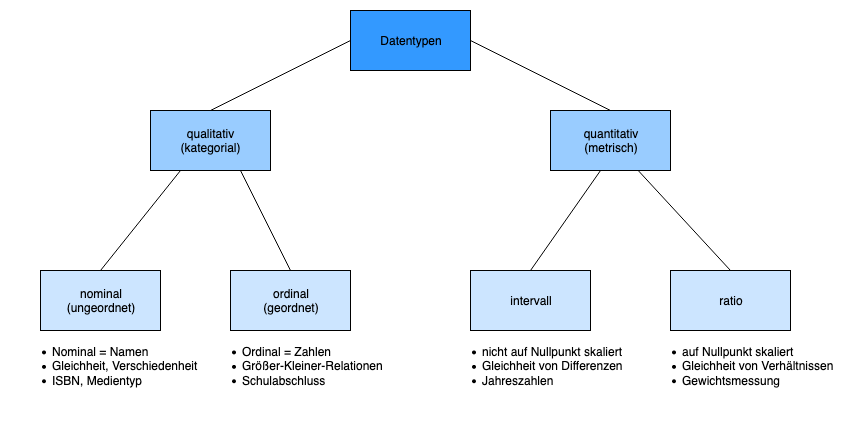
\includegraphics[width=12cm]{dt}
        \caption{Statistische Datentypen mit Aussagegehalten und Beispielen}
        \label{fig:data types}
\end{figure}


%Nominale Datentypen können auch Ziffern beinhalten. 
Unterschieden werden die Merkmale ferner nach diskret und stetig.
Ein diskretes Merkmal kann auf der Basis der natürlichen Zahlen abzählbar viele Merkmalsausprägungen annehmen.
Die Größe des Medienbestandes einer Bibliothek ist ein diskretes Merkmal, da es keine halben oder viertel Medien gibt.
Im Gegensatz dazu können die Merkmalsausprägungen eines stetigen Merkmals jeden beliebigen Wert annehmen. Die Raumtemperatur ist ein stetiges Merkmal.
Qualitative Merkmale können nur diskret sein, während quantitative Merkmale sowohl diskret als auch stetig sein können. 
Für kategoriale Merkmale eignen sich Balken und Kreisdiagramme eher als Liniendiagramme, da kategoriale Daten nur diskret sein können.
%Für quantitative Merkmale eignen sich  Balken- und Liniendiagramme???

Der Einsatz von infrage kommenden Datenvisualisierungen wird ebenfalls bestimmt von der Größe der Datenmenge.
Die Darstellung einer großen Datenmenge kann zum Beispiel durch die falsche Wahl des Diagramms überladen wirken. 
So kann die Darstellung einer Datenmenge mit vielen Kategorien durch Balken- und Kreisdiagramme 
in der Übersichtlichkeit leicht an Grenzen stoßen und den Wert der zu erzielenden Aussage verwischen.

%Es ist zu letztlich zu überlegen, welcher Art von Beziehung zwischen den Daten gezeigt werden soll. die Auswertung der Daten verfolgt und
Letztlich ist zu überlegen, für wen die Daten mit grafischen Elementen präsentiert werden. Davon hängt auch ab, 
mit welchen Schwerpunkten Merkmale und Eigenschaften präsentiert werden sollen \cite[vgl.][17]{kirk_data_2019}. 

Die Präsentation der Daten zu wem ... umschließt Interaktivität -> statischen Bildern hinzu interaktiven \dots
audience
Neuere Entwicklung gehen hinzum Dashboard  - einer Darstellung der wesentlichen Informationen komprimiert \dots
Dashboards können  als Teil von Business-Intelligence-Systemen verstanden werden.


\section{Business-Intelligence-Systeme}

\cite{kemper_business_2010}
\cite{gluchowski_management_2008}
Vielfältige Definition:
Bi-Def.:
Business-Intelligence-Systeme stellen ein ganzheitliches System dar. Sie sind ein
integrierter, unternehmensspezifischen, IT-basierten Gesamtansatz zur Unterstützung betrieblicher Entscheidungen dar.
\cites[vgl.][5]{muller_business_2013}[vgl.][270]{abts_grundkurs_2017}
Als Datenlieferanten für BI-Systeme dienen die operativen Anwendungssysteme.
Historisch fällt die Entstehung des Begriffs mit der Entwicklung Data-Ware-Houses für unternehmerische Zwecke zusammen.
Der Aufbau widerspiegelt sich in der Referenzarchitektur

Daten werden aus den operativen Daten und externen Datenquellen extrahiert und durch Transformation, Aggregation, Gruppierung
und Speicherung durch OLAP-Operatoren oder SQL-Aggregatfkt. abgeleitet.
Daten werden Auswertungsvcverfahren wie der Statistik, d.h. Schätz- und Testverfahren, des Data Minings auf interessante Abhängigkeiten analysiert, visualisiert
und den Stakeholdern bereitgestellt. Dies geschieht mit Dashboards oder BI-Portalen.
\cite[vgl.][5]{muller_business_2013}


\cite{abts_grundkurs_2017}.  
Zielgruppe: Management auf allen Ebenen
BI muss unternehmensspezifisch angepasst werden
integriert: Bereitstellung unters. Daten (interne, externe, operative und analytische)
    Anwendung unters. Methoden (stat. Methoden)
    Bereitstellung und Verteilumg der Analyseergebnisse umfasst. -> Portale, dashboardsBI-Systeme können extensional beschrieben werden, da sie
sich nicht nur auf einen unternehmerischen Bereich zentrieren. Im Zentrum der BI-Systeme steht das Data-Ware-House, was\cite{muller_business_2013}

Überleitung BI-Lösungen sind auch schon im Bibliothekswesen vereinzelt angekommen.
Seit dem Aufkommen der \acrfull{BI} in den 1990 er Jahren, sind eine Vielzahl von Begriffsdefinitionen entstanden.
Diese Begriffsdefinitionen unterscheiden sich mmanchmal nur 
Historisch eng verwachsen sind BI-Systeme mit dem Aufkommen des Konze
Zwei Hauptmerkmale: dass sie das Management unterstützen sollen. \cite{linden_geschaftsmodellbasierte_2016}
Abgrenzung zu operativen Systemen, von denen Business Intelligent-Systeme die Daten erhalten \cite{abts_grundkurs_2017}.

Intelligence wird dabei als Geschäftsinformation oder Informaion verstanden.\cite{linden_geschaftsmodellbasierte_2016}
Grundlage der BI-Systeme sind die Daten aus dem operativen Systemen. Diese werden mit dem Prozess Extracxt, Transform and Load (ETL) in ein 
Data Ware House geladen. 

Aufbau 


Die Entwicklung IT-unsterstützender Systeme fängt in den 1960er Jahren an.
\acrfull{DWH}\\
In dem Zusammenhang bit BI bedeuted Data Ware House eine themenorientierte, vereinheitlichte, beständige, zeitbezogene
Sammlung von Daten zur Unterstützung von Managemententscheidungen\cite[vgl.][271]{abts_grundkurs_2017}

Data Lake:


Dashboards:\\
Nach Few
\textquote{A dashboard is a visual display of the most important information needed to achieve one or more objectives; consolidated and arranged on a single screen so the
information can be monitored at a glance.}\cite{few_information_2006}


Historisch gesehen seit den 1960 er Jahren. Erst im Zuge der Durchsetzung leistungsfähiger Rechner können große Datenmengen analysiert werden
Definition Business-Intelligence\\
4 Sätze

Historie
2 Sätze

Aufbau der Architektur 

operative Datenbestände -> Datenbereitstellung -> Datenanalyse -> Zugriff, Präsentation
im herkömmlichen Sinne werden datenbanken als dataware houses -> datenanalysen betrieben -> präsentiert

Darunterliegende System
ETL 5 bis 10 Sätze
zu den einzelnen Phasen
3- 4 Sätze
Abbildung

Dashboard
3 Sätze

BI bezeichnet einen integrierten, unternehmensspezifischen, IT-basierten Gesamtansatz zur betrieblichen Entscheidungsunterstützung.
BI bezeichnet einen integrierten, unternehmensspezifischen, IT-basierten Gesamtansatz zur betrieblichen Entscheidungsunterstützung.
BI bezeichnet einen integrierten, unternehmensspezifischen, IT-basierten Gesamtansatz zur betrieblichen Entscheidungsunterstützung.
BI bezeichnet einen integrierten, unternehmensspezifischen, IT-basierten Gesamtansatz zur betrieblichen Entscheidungsunterstützung.
BI bezeichnet einen integrierten, unternehmensspezifischen, IT-basierten Gesamtansatz zur betrieblichen Entscheidungsunterstützung.
BI bezeichnet einen integrierten, unternehmensspezifischen, IT-basierten Gesamtansatz zur betrieblichen Entscheidungsunterstützung.
BI bezeichnet einen integrierten, unternehmensspezifischen, IT-basierten Gesamtansatz zur betrieblichen Entscheidungsunterstützung.
BI bezeichnet einen integrierten, unternehmensspezifischen, IT-basierten Gesamtansatz zur betrieblichen Entscheidungsunterstützung.
BI bezeichnet einen integrierten, unternehmensspezifischen, IT-basierten Gesamtansatz zur betrieblichen Entscheidungsunterstützung.
BI bezeichnet einen integrierten, unternehmensspezifischen, IT-basierten Gesamtansatz zur betrieblichen Entscheidungsunterstützung.
BI bezeichnet einen integrierten, unternehmensspezifischen, IT-basierten Gesamtansatz zur betrieblichen Entscheidungsunterstützung.
BI bezeichnet einen integrierten, unternehmensspezifischen, IT-basierten Gesamtansatz zur betrieblichen Entscheidungsunterstützung.
BI bezeichnet einen integrierten, unternehmensspezifischen, IT-basierten Gesamtansatz zur betrieblichen Entscheidungsunterstützung.
BI bezeichnet einen integrierten, unternehmensspezifischen, IT-basierten Gesamtansatz zur betrieblichen Entscheidungsunterstützung.
BI bezeichnet einen integrierten, unternehmensspezifischen, IT-basierten Gesamtansatz zur betrieblichen Entscheidungsunterstützung.
BI bezeichnet einen integrierten, unternehmensspezifischen, IT-basierten Gesamtansatz zur betrieblichen Entscheidungsunterstützung.
BI bezeichnet einen integrierten, unternehmensspezifischen, IT-basierten Gesamtansatz zur betrieblichen Entscheidungsunterstützung.
BI bezeichnet einen integrierten, unternehmensspezifischen, IT-basierten Gesamtansatz zur betrieblichen Entscheidungsunterstützung.
BI bezeichnet einen integrierten, unternehmensspezifischen, IT-basierten Gesamtansatz zur betrieblichen Entscheidungsunterstützung.
BI bezeichnet einen integrierten, unternehmensspezifischen, IT-basierten Gesamtansatz zur betrieblichen Entscheidungsunterstützung.
BI bezeichnet einen integrierten, unternehmensspezifischen, IT-basierten Gesamtansatz zur betrieblichen Entscheidungsunterstützung.
BI bezeichnet einen integrierten, unternehmensspezifischen, IT-basierten Gesamtansatz zur betrieblichen Entscheidungsunterstützung.
BI bezeichnet einen integrierten, unternehmensspezifischen, IT-basierten Gesamtansatz zur betrieblichen Entscheidungsunterstützung.
BI bezeichnet einen integrierten, unternehmensspezifischen, IT-basierten Gesamtansatz zur betrieblichen Entscheidungsunterstützung.

\clearpage
Speist sich aus folgenden Stages\\
Bild\\

Bi-Ordnungsrahmen bestehend aus
Datenbereitstellung,
              Generierung der konsistetenten und stimmigen Daten aus dem Quellsystem
 
12          Datawarehouse-Konzepte
Informationsgenerierung
              Analysesysteme
13
Informationszugriff
              Komfortable Benutzerschnittstellen
              Single-Sign-On

ETL
KDD
Data Mining
Dashbords 


Was sind Business-Intelligence-Löungen?\\
%Wo kommen Buisiness-Intelligence-Lösungen zum Einsatz zum Einsatz?
Es gibt eine Vielzahl kommerzieller Lösungen für den Bibliotheksbereich, die auf Business-Intelligence-Systemen basieren.
Zu nennen wären \textit{AlmaAnalytics} für das Next-Generation-Library-System \textit{Alma} von \textit{ExLibris}\footnote{\url{https://www.exlibrisgroup.com/products/alma-library-services-platform/alma-analytics}

Stand: 26.05.2020}, \textit{BibControl} von \textit{OCLC}\footnote{\url{https://www.oclc.org/de/bibcontrol.html} Stand: 26.05.2020},
\textit{CollectionHq} von \textit{Baker \& Taylor}\footnote{\url{https://www.collectionhq.com/} Stand: 26.05.2020} oder \textit{Libinsight} von \textit{SpringShare}\footnote{\url{https://springshare.com/libinsight/} Stand: 26.05.2020}.
Darüber hinaus gibt es Business-Intelligence-Applikationen, die von
Bibliotheken für Reporting, Datenanalyse und Datenvisualisierung adaptiert werden,
wie zum Beispiel \textit{Tableau} von der Firma \textit{Tableau Software} oder
\textit{Crystal Reports} von \textit{SAP}.
Diese Applikationen sind entweder
an bestimmte Bibliothekssysteme zurückgebunden, limitiert in ihren
Funktionen\cite{golas_statistische_2018} oder zu generisch.
Überdies wird sowohl von \textit{HeBis} bzw. von der
Lokal-Bibliothekssystembetreuung als auch von der \textit{mpdl} keine Applikation
in dieser Richtung angeboten.
Ebenso ist ungewiss, wann die Ablösung des schon betagten \textit{CBS/LBS} hin zu
einem neuen Next-Generation-Library-System im \textit{HeBis-Verbund} stattfinden wird und ob
es ein Modul zur statistischen Datenerhebung liefern wird.
